\documentclass[a4paper, 12pt]{article}

\usepackage{enumerate}
\usepackage{hyperref}
\hypersetup{
	colorlinks=true,
	linkcolor=blue,
	filecolor=blue,
	urlcolor=blue,
	citecolor=blue,
}
\usepackage{amsmath}
\usepackage{amsthm}
\usepackage{amssymb}
\usepackage[margin=3cm]{geometry}
\usepackage{mathpazo}
\usepackage{url}
\usepackage{subcaption}
\usepackage{tikz}
\usepackage{pgf}
\usepackage{longtable}
\usepackage{multirow}
\usepackage{graphicx}
\usepackage{pgfplots}
\usepackage{cleveref}
\usepackage{amsrefs}
\usepackage{bbm}
\usepackage{csquotes}
\usepackage{wrapfig}
\usepackage{algorithm}
\usepackage{algpseudocode}
\usepackage{mathrsfs}
\usepackage{afterpage}

\numberwithin{equation}{section}
\numberwithin{figure}{section}

\newtheorem{thm}{Theorem}[section]
\newtheorem*{thm*}{Theorem}
\newtheorem*{con*}{Conjecture}
\newtheorem{lem}[thm]{Lemma}
\newtheorem{prop}[thm]{Proposition}
\newtheorem{cor}[thm]{Corollary}
\newtheorem{lemma}[thm]{Lemma}
\newtheorem{conj}[thm]{Conjecture}

\theoremstyle{definition}
\newtheorem{defn}[thm]{Definition}
\newtheorem{remark}[thm]{Remark}
\newtheorem{ex}[thm]{Example}
\newtheorem{quest}[thm]{Question}
\newtheorem{obs}[thm]{Observation}

\renewcommand{\leq}{\leqslant}
\renewcommand{\geq}{\geqslant}
\newcommand{\N}{\mathbb{N}}
\newcommand{\Z}{\mathbb{Z}}
\newcommand{\Q}{\mathbb{Q}}
\newcommand{\R}{\mathbb{R}}
\newcommand{\C}{\mathbb{C}}
\newcommand{\tr}{\mathrm{t}}
\newcommand{\WEEK}[1]{%
\hfill Week #1

\vspace{-1em}

\begin{center}
	\rule{\textwidth}{2pt}
\end{center}
\vspace{0.5em}%
}

\renewcommand{\algorithmicrequire}{\textbf{Input:}}
\renewcommand{\algorithmicensure}{\textbf{Output:}}

% Configure comments to flush right
\renewcommand{\algorithmiccomment}[1]{\hfill \# #1}

\setcounter{tocdepth}{2}

\allowdisplaybreaks

\title{Geometric Foundations of Data Analysis I}
\author{Joshua Maglione}
\date{\today}

\begin{document}

\maketitle
\tableofcontents

\setcounter{section}{3}
\setcounter{algorithm}{1}


\section{Clustering}

Similar to PCA, clustering is a way to understand structure of data. Clustering
or cluster analysis is a generic term for algorithms designed to partition a
given data into clusters. Clusters is a word that does not really have a precise
meaning, and its meaning might even depend on situation, but generally we
intuitively understand that clusters are groups of data points as seen in
\Cref{fig:clusters}.

\begin{figure}
	\centering 
	\begin{tikzpicture}
		% Cluster 1
		\foreach \x/\y in {1.2/2.3, 1.5/1.8, 2.0/2.5, 1.8/2.0, 2.5/2.7}
			\fill[orange] (\x, \y) circle (2pt);
		
		% Cluster 2
		\foreach \x/\y in {3.5/4.0, 3.7/3.8, 4.0/4.5, 4.2/4.2, 3.8/4.8}
			\fill[blue] (\x, \y) circle (2pt);
		
		% Cluster 3
		\foreach \x/\y in {6.0/5.5, 5.5/5.0, 6.2/5.8, 5.8/6.2, 6.5/6.0}
			\fill[purple] (\x, \y) circle (2pt);

		% Cluster 4
		\foreach \x/\y in {7.0/3.5, 8.0/3.0, 7.5/4.0, 7.8/4.2, 8.2/3.8}
			\fill[teal] (\x, \y) circle (2pt);
		
		% Axis
		\draw[->] (0,0) -- (9,0) node[right] {$x$};
		\draw[->] (0,0) -- (0,7) node[above] {$y$};
	\end{tikzpicture}
	\caption{Data points in $\R^2$ that form four clusters.}
	\label{fig:clusters}
\end{figure}

Clustering is a fantastic tool for answering certain kinds of questions about
the data like the following.
\begin{itemize}
	\item What sub-populations exist in the data? 
	\item Are there outliers? 
	\item Are the sub-populations cohesive or can they be partitioned further? 
\end{itemize}
``Populations'' presupposes a certain perspective that need not be true. For
example, clustering algorithms are used on gene sequences in medicine and
biological sciences. See for example the hierarchical clustering done on
sequences of genes for breast cancer in \Cref{fig:clustering-genes}.

\begin{figure}[h]
	\centering
	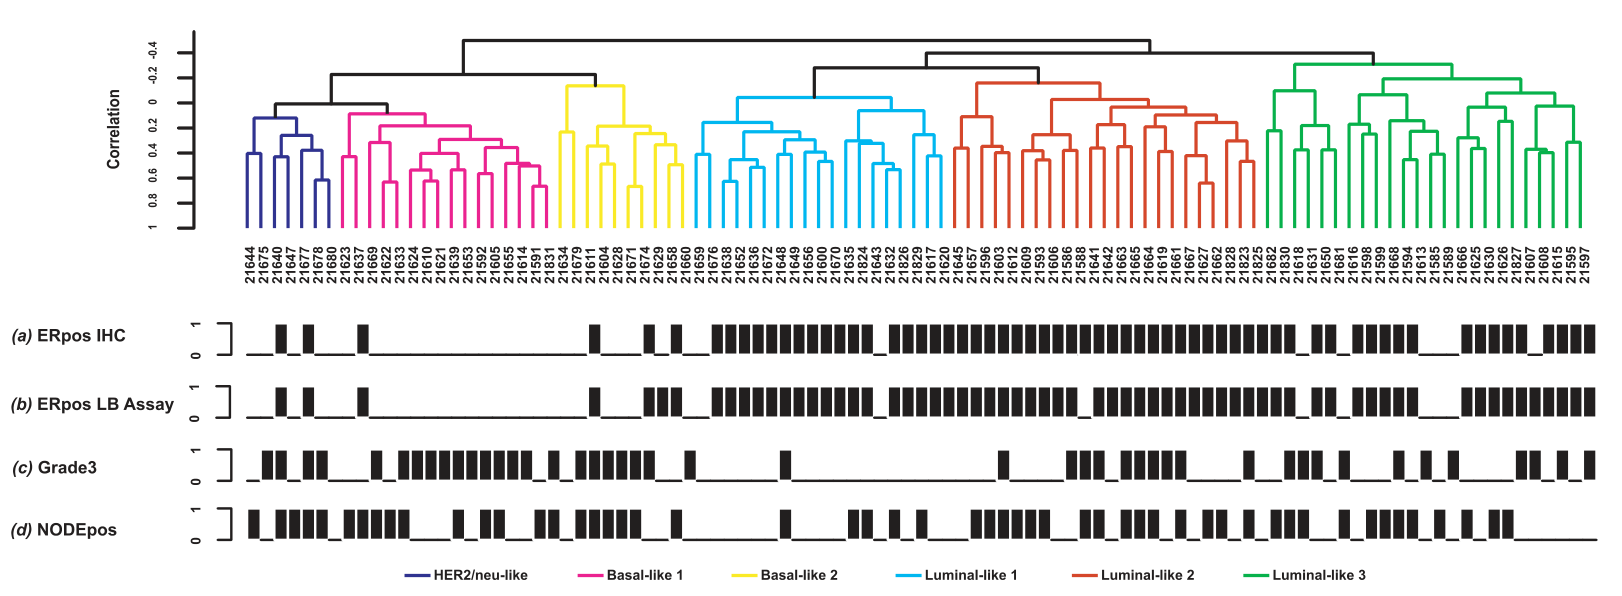
\includegraphics[scale=0.4]{graphics/clustering-in-medicine.png}
	\caption{A hierarchical figure taken from \cite{BreastCancer}. The clusters are seen with the different colours.}
	\label{fig:clustering-genes}
\end{figure}

Clustering is also one of the first steps in machine learning---an example of
unsupervised learning. This just means that the machine ``learns'' of patterns
and structures from the unlabeled data. Sometimes data are put into clusters,
and then nearly all of the data, except for the cluster ID is discarded, which
can save significant space in the analysis stage. To quote Google \cite{Google}:

\begin{displayquote}
	At Google, clustering is used for generalization, data compression, and
	privacy preservation in products such as YouTube videos, Play apps, and
	Music tracks.
\end{displayquote}

There is no one clustering algorithm that is optimal in every situation; in
fact, because data can cluster in many different ways, one needs a whole
clustering toolkit. We will talk about two common methods for clustering:
\textit{$k$-means} and \textit{single linkage} clustering. At the core of both
of these clustering algorithms is a different assumption on the definition of a
cluster. 

\subsection{Introduction to $k$-means clustering}

The idea around $k$-means clustering is incredibly simple: group the data into
$k$ clusters based on the shortest distance to the center of the cluster. From
this, we see how ``cluster'' is interpreted in the $k$-means algorithm---a
cluster forms a ``cell'' in Euclidean space and data points outside of this cell
are outside of the cluster. The shape of these cells depend on the layout of the
centers of the clusters. 

Before we go through the algorithm for $k$-means clustering, let's explore some
of the many applications of this algorithm. 

\subsection{Image compression with $k$-means}

Suppose we have a \texttt{jpg} file that is $m\times n$ pixels. We can turn this
image file into a $3$-dimensional array, namely an $m\times n\times 3$ array.
Alternatively, we can interpret this as three $m\times n$ matrices corresponding
to the red, green, and blue values of the image. 

\begin{wrapfigure}{r}{6cm}
	\centering
	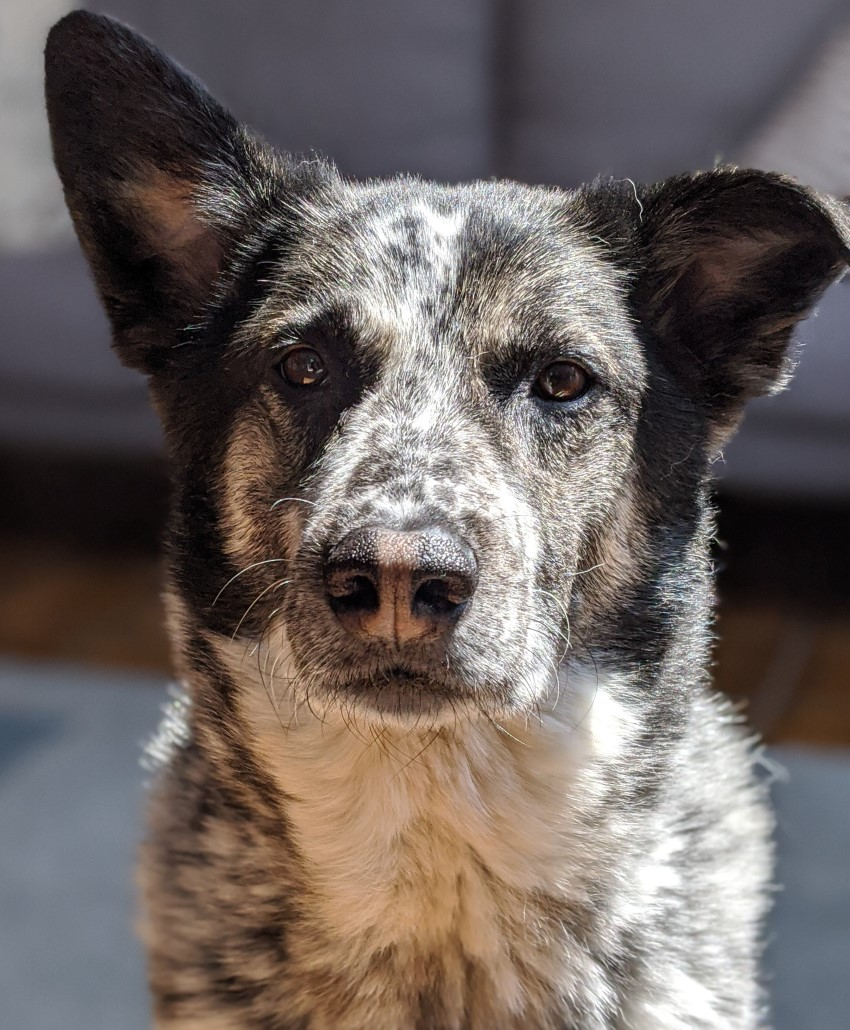
\includegraphics[scale=0.20]{graphics/Sherlock.jpg}
	\caption{Sherlock.}
	\label{fig:sherlock}
\end{wrapfigure}
We can use $k$-means clustering by interpreting each pixel as a data point in
$\R^3$ and determining clusters. Once we find our clusters, we can replace all
the pixels with the center it is closest to. The impact is that we replace all
the different colours with exactly $k$ colours---essentially compressing the
image. 

Let's see how this might look on one of my photos. Meet my dog, Sherlock; he is
depicted in \Cref{fig:sherlock}. There is not very many colours in the image, so
we should expect that low values of $k$ will produce an image that looks fairly
similar. Running a $k$-means clustering for each $k\in \{2,\dots, 10\}$ yields
nine different images seen in \Cref{fig:k-means-sherlock}.

\begin{figure}[h]
	\centering
	% \vspace{-2em}
	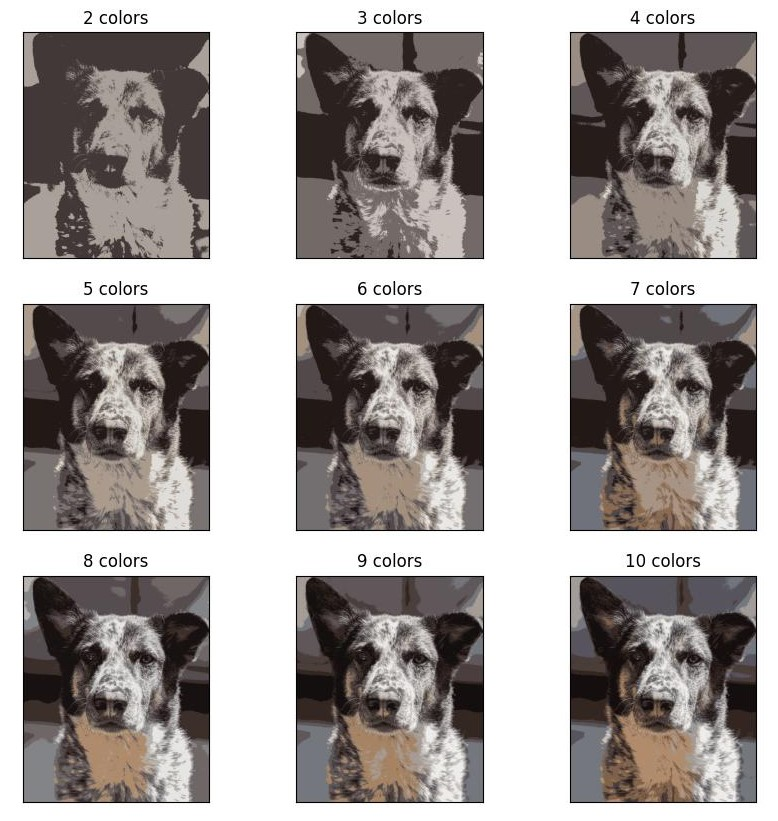
\includegraphics[scale=0.75]{graphics/k_means_Sherlocks.jpg}
	\caption{$k$-means clustering on the image in \Cref{fig:sherlock}.}
	\label{fig:k-means-sherlock}
\end{figure}

\subsection{The $k$-means algorithm}

There are many versions of the basic algorithm we will describe. We use
pseudo-code to give the details of the algorithm; this is a way of giving the
idea of the structure of the code without diving into the specifics of any
particular language. 

We provide pseudo-code for a basic $k$-means algorithm in \Cref{alg:k-means}.
The algorithm returns a function $\Lambda : \{1,\dots, n\} \to \{1,\dots, k\}$,
which can be interpreted as a label for the $n$ data points. The algorithm
accomplishes this by randomly choosing the $k$ centroids, and then clustering
the data points accordingly. Once all the data points have been labeled, we
recompute the centroids by taking the mean point of all the data points in a
given cluster to be the new centroid. 

\begin{algorithm}
	\caption{(Basic) $k$-means}\label{alg:k-means}
	\begin{algorithmic}[1]
		\Require a positive integer $k$ and $n$ data points $x_i\in\R^m$,
		\Ensure a map $\Lambda : \{1,\dots,n\} \to \{1,\dots, k\}$.
		\State Randomly assign the $k$ centroids $c_i$ to $k$ data points.
		\State Let $\Lambda_0$ and $\Lambda$ be constant functions mapping to $-1$ and $0$, respectively.
		\While{$\Lambda_0 \neq \Lambda$}
			\State Set $\Lambda_0 = \Lambda$.
			\For{$i\in \{1,\dots,n\}$}
				\State Set $\Lambda(i) = j$ if $\|x_i-c_j\| = \min\{\|x_i-c_r\| : 1\leq r \leq k\}$.
			\EndFor
			\For{$i\in \{1,\dots, k\}$}
				\State Set $c_i = \left(\sum_{j \in \Lambda^{-1}(i)} x_j\middle) \right/ \# \left(\Lambda^{-1}(i)\right)$.
			\EndFor
		\EndWhile
		\State \Return $\Lambda$.
	\end{algorithmic}
\end{algorithm}

In the first step of $k$-means (see line 1 in \Cref{alg:k-means}), we randomly
assign the $k$ centroids. For different initial assignments, one can get
different outputs. This is like trying to find global extrema on a ``bumpy''
graph by starting at a random point on the graph and then looking for the
nearest local extrema. There are a number of ways to improve the $k$-means
algorithm, we will not cover them, but many consider different variations for
their specific data at hand. 

\subsection{A small example with $k$-means}

We will consider 40 points in $\R^2$, which can be seen in \Cref{fig:4-means},
and we will look for $4$ clusters. You might try to see how you would cluster
the data. 

\begin{figure}[h]
	\centering 
	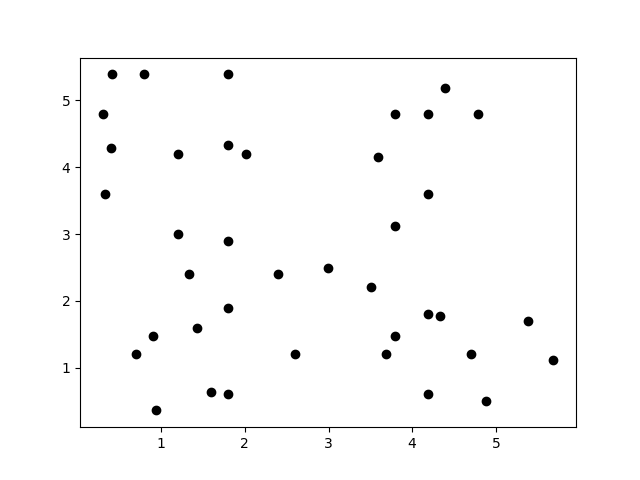
\includegraphics[scale=0.6]{graphics/k_means_iter-1.png}
	\caption{The plotted data we will use to run a $4$-means clustering.}
	\label{fig:4-means}
\end{figure}

We will randomly select four data points for our initial centroids, and then we
will group the data points into the four clusters. We will show this by
colouring the Voronoi cells different colours and indicating the centroids by
white crosses. All of the iterations of one $k$-means algorithm can be seen in
\Cref{fig:4-means-iterations}. Just to illustrate how sensitive $k$-means is to
the initial choice of centroids, we run the algorithm again in
\Cref{fig:4-means-iterations-alt}.



% \afterpage{\clearpage}

\begin{figure}[ht]
	\centering 
	\begin{subfigure}[b]{0.49\textwidth}
		\centering 
		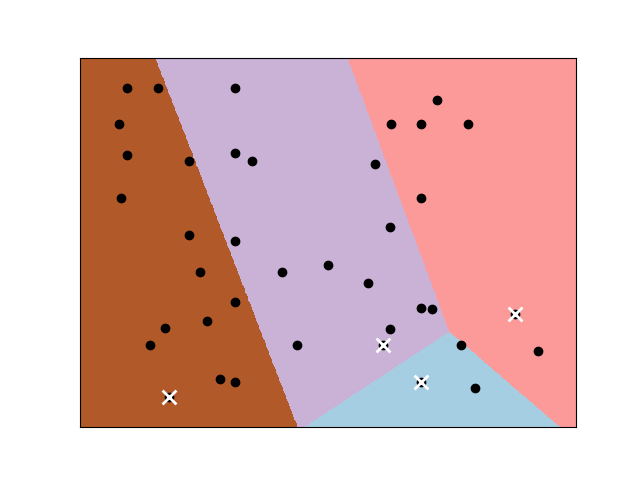
\includegraphics[scale=0.4]{graphics/k_means_iter0.png}
		\vspace{-0.75em}
		\caption{Iteration 0}
	\end{subfigure}~%
	\begin{subfigure}[b]{0.49\textwidth}
		\centering 
		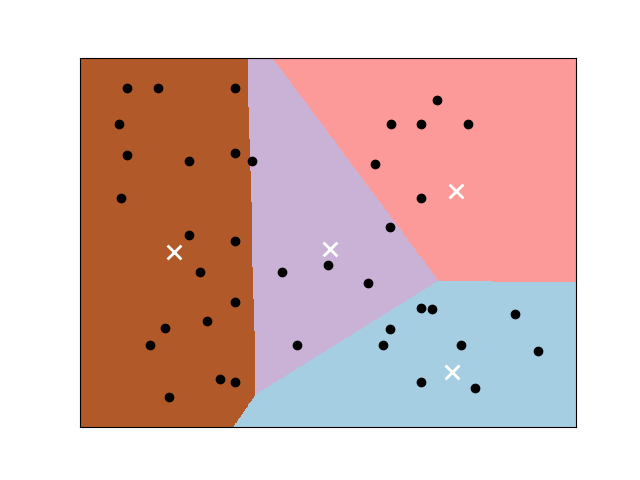
\includegraphics[scale=0.4]{graphics/k_means_iter1.png}
		\vspace{-0.75em}
		\caption{Iteration 1}
	\end{subfigure}
	\begin{subfigure}[b]{0.49\textwidth}
		\centering 
		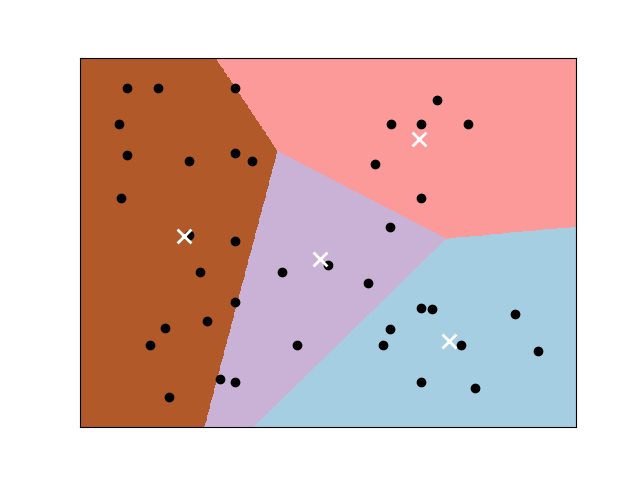
\includegraphics[scale=0.4]{graphics/k_means_iter2.png}
		\vspace{-0.75em}
		\caption{Iteration 2}
	\end{subfigure}~%
	\begin{subfigure}[b]{0.49\textwidth}
		\centering 
		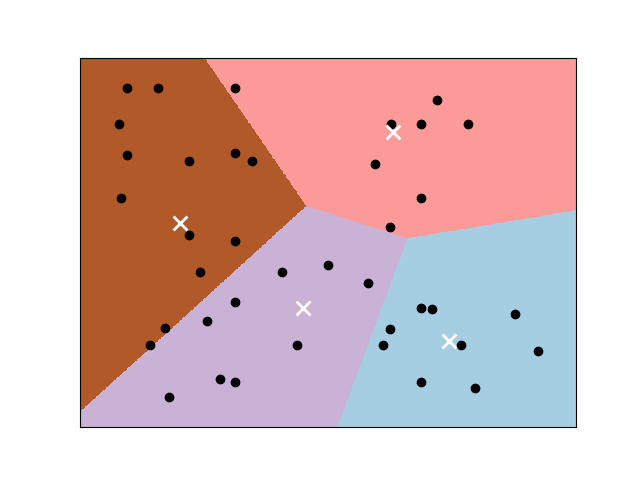
\includegraphics[scale=0.4]{graphics/k_means_iter3.png}
		\vspace{-0.75em}
		\caption{Iteration 3}
	\end{subfigure}
	\begin{subfigure}[b]{0.49\textwidth}
		\centering 
		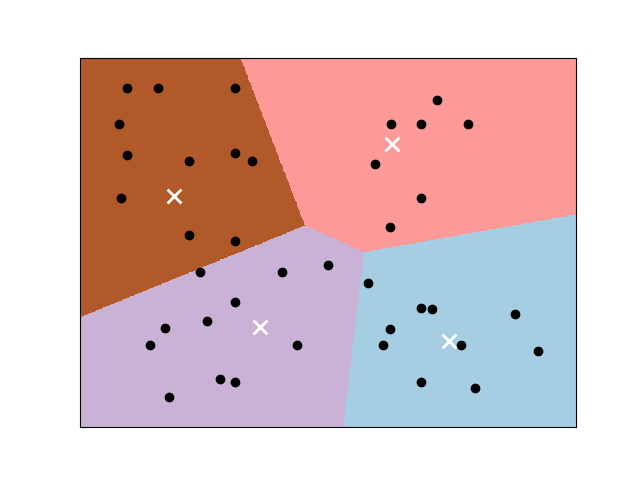
\includegraphics[scale=0.4]{graphics/k_means_iter4.png}
		\vspace{-0.75em}
		\caption{Iteration 4}
	\end{subfigure}~%
	\begin{subfigure}[b]{0.49\textwidth}
		\centering 
		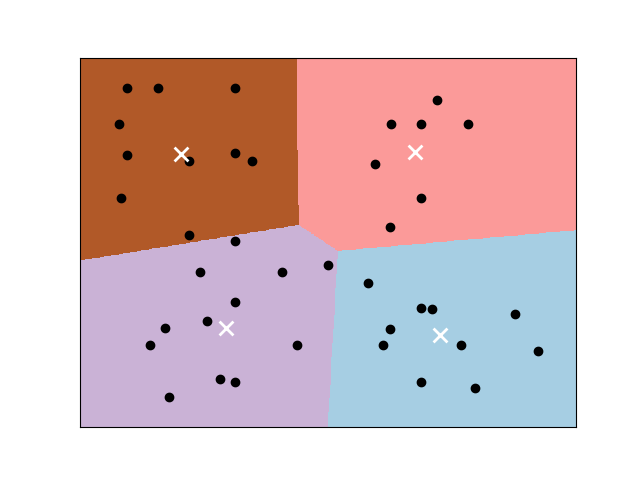
\includegraphics[scale=0.4]{graphics/k_means_iter5.png}
		\vspace{-0.75em}
		\caption{Iteration 5}
	\end{subfigure}
	\begin{subfigure}[b]{0.66\textwidth}
		\centering 
		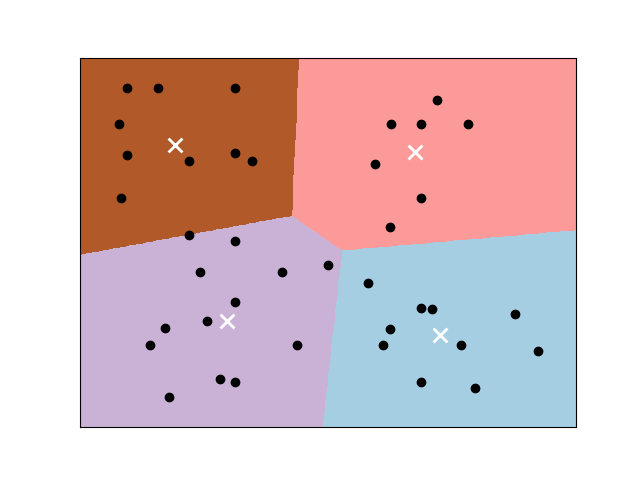
\includegraphics[scale=0.4]{graphics/k_means_iter6.png}
		\vspace{-0.75em}
		\caption{Iteration 6}
	\end{subfigure}
	\caption{Seven iterations of one $k$-means algorithm.}
	\label{fig:4-means-iterations}
\end{figure}

\begin{figure}[t]
	\centering 
	\begin{subfigure}[b]{0.49\textwidth}
		\centering 
		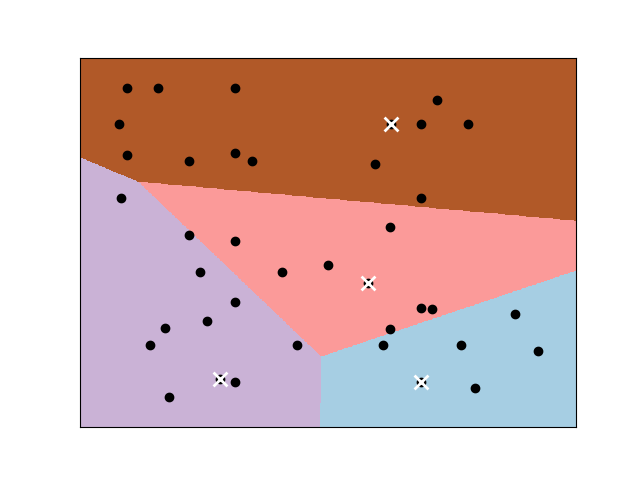
\includegraphics[scale=0.4]{graphics/k_means_iter0_alt.png}
		\vspace{-0.75em}
		\caption{Iteration 0}
	\end{subfigure}~%
	\begin{subfigure}[b]{0.49\textwidth}
		\centering 
		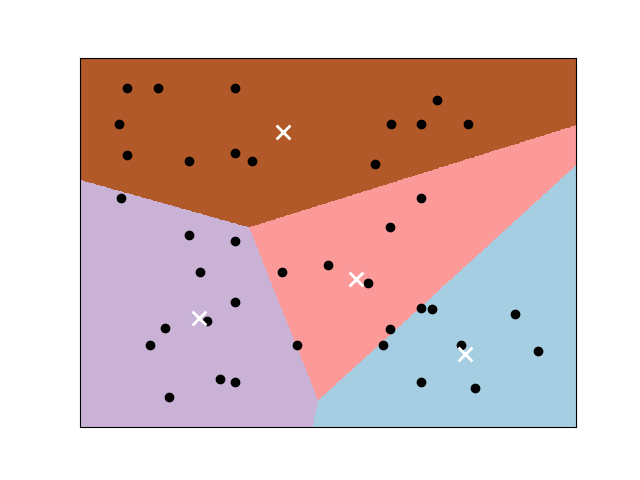
\includegraphics[scale=0.4]{graphics/k_means_iter1_alt.png}
		\vspace{-0.75em}
		\caption{Iteration 1}
	\end{subfigure}
	\begin{subfigure}[b]{0.49\textwidth}
		\centering 
		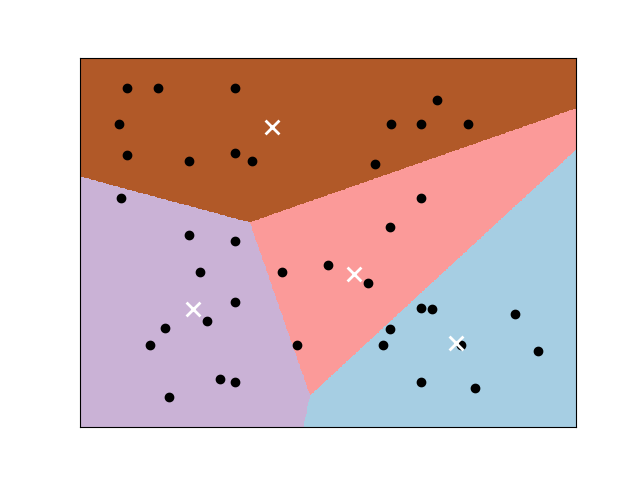
\includegraphics[scale=0.4]{graphics/k_means_iter2_alt.png}
		\vspace{-0.75em}
		\caption{Iteration 2}
	\end{subfigure}~%
	\begin{subfigure}[b]{0.49\textwidth}
		\centering 
		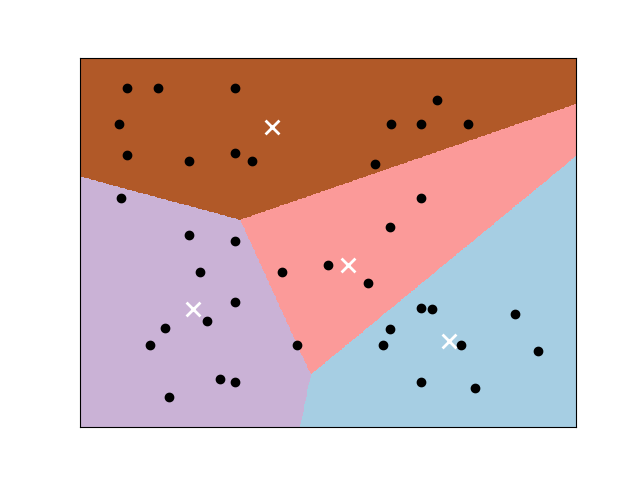
\includegraphics[scale=0.4]{graphics/k_means_iter3_alt.png}
		\vspace{-0.75em}
		\caption{Iteration 3}
	\end{subfigure}
	\caption{Four iterations of another $k$-means algorithm.}
	\label{fig:4-means-iterations-alt}
\end{figure}

\subsection{Introduction to hierarchical clustering}

Hierarchical clustering is, in some sense, the opposite approach to clustering
than $k$-means. We will primarily be working with Single-linkage clustering.
Single-linkage or, more generally, \emph{neighbour joining} clustering is a
hierarchical clustering algorithm. With $k$-means, we need to give the number of
clusters $k$ in order to run the algorithm. With neighbour joining, we look at
all the possible clusterings under prescribed conditions by means of a
\emph{dendrogram}. We have already seen an example of the output of a
hierarchical clustering algorithm; see \Cref{fig:clustering-genes}.

The basic idea of neighbour joining clustering is that every data point is its
own cluster and under certain conditions, two clusters are merged at each step
until all points are in one cluster. The output is not a specific clustering of
the data, but rather all the possible clusterings. This is communicated through
a dendrogram. 

Before we look at the algorithm, let's consider a specific application.

\subsection{An application of hierarchical clustering}

We will look at the study in~\cite{BreastCancer} a little closely; see also
\Cref{fig:clustering-genes}. People diagnosed with breast cancer can have very
different clinical outcomes. We do not really know why this is the case, but one
suggestion might be that our knowledge of the specific breast cancer tumors is
lacking. Sotiriou et al.~\cite{BreastCancer} propose clustering the tumors by
gene expression profiles, via unsupervised hierarchical clustering. 

Prior to their work, the tumors could be partitioned into two major subgroups
based on their estrogen receptors. Using clustering methods, Sotiriou et al.
were able to obtain this partition at the top of the dendrogram---if one cuts it
so there are exactly two clusters, these align with the two subgroups based on
estrogen receptors. They were able to further partition the two subgroups based
on their basal and luminal characteristics. This led to the six clusters
(represented by different colours) in \Cref{fig:clustering-genes}. This is also
in line with previous work done by different research teams, and offers more
evidence that their hypothesis is correct---that breast cancer tumors ought to
be clustered in the established way.

\subsection{The neighbour joining algorithm}

We will describe a class of \emph{agglomerative} algorithms that can be altered
to produce different outcomes based on certain given conditions. In order to do
this, one of the inputs is a distance function, which can be obtained from a
\emph{metric}. We want the metric to be defined on finite subsets of $\R^m$,
which will be interpreted as clusters in the actual algorithm. 

\begin{defn}
	A function $d: \mathscr{M}\times \mathscr{M} \to \R$ on a set $\mathscr{M}$
	is a \emph{metric} if 
	\begin{enumerate}
		\item for all $X, Y\in \mathscr{M}$, we have $d(X, Y) \geq 0$, where
		equality holds if and only if $X=Y$,
		\item for all $X, Y\in\mathscr{M}$, we have $d(X, Y) = d(Y, X)$, and
		\item for all $X, Y, Z\in\mathscr{M}$, the triangle inequality is
		satisfied:
		\[ 
			d(X, Y) + d(Y, Z) \geq d(X, Z). 
		\] 
	\end{enumerate}
	Functions satisfying (1) and (2) are called \emph{semimetrics}. 
\end{defn}

\begin{lem}\label{lem:semimetrics}
	The Euclidean distance $d(x,y) = \|x-y\|$ is a metric on $\R^m$. The square
	of the Euclidean distance, $d_{\square}(x,y)=\|x-y\|^2$, is not a metric but
	a semimetric.
\end{lem}

\begin{proof}
	To show that $d_{\square}$ does not satisfy the triangle inequality, let
	$a\in\R$ be positive. Then $|-a|^2 + |a|^2 < |2a|^2$, so
	\begin{align*}
		d_{\square}(a,0) + d_{\square}(-a,0) &< d_{\square}(a,-a). \qedhere
	\end{align*}
\end{proof}

In the context of clustering, having a metric is not necessary. For example,
because $x\mapsto x^2$ is monotonically increasing on the $\R_{\geq 0}$, it
follows that $d(x,y) < d(u,v)$ if and only if $d_{\square}(x,y) <
d_{\square}(u,v)$; here we are using the notation from \Cref{lem:semimetrics}.
Thus, it is irrelevant if we cluster two points based on $d$ or $d_{\square}$,
so we allow our distance functions to come from semimetrics. 

Let's write $\mathscr{F}_m$ for the set of finite subsets of $\R^m$, so we will
describe a few distance functions on $\mathscr{F}_m$.
\begin{description}
	\item[Single-linkage:] For $C_1,C_2\in\mathscr{F}_m$, 
	\begin{align*}
		d(C_1, C_2) &= \min\left\{ \| x - y\| : x\in C_1, y\in C_2 \right\}. 
	\end{align*}
	\item[Complete-linkage:] For $C_1,C_2\in\mathscr{F}_m$, 
	\begin{align*}
		d(C_1, C_2) &= \max\left\{ \| x - y\| : x\in C_1, y\in C_2 \right\}. 
	\end{align*}
	\item[Average-linkage:] For $C_1,C_2\in\mathscr{F}_m$, 
	\begin{align*}
		d(C_1, C_2) &= \dfrac{1}{\# C_1 \cdot \# C_2} \sum_{x \in C_1} \sum_{y\in C_2} \|x - y\|. 
	\end{align*}
\end{description}
Technically the single-linkage is not a semimetric: if $C_1\cap C_2\neq
\varnothing$ yet $C_1\neq C_2$, then $d(C_1, C_2)=0$. However we only consider
sets $C_1$ and $C_2$ with trivial intersection anyways, so this problem is
avoided. 

\begin{lem}
	The complete-linkage function defines a metric on $\mathscr{F}_m$.
\end{lem}

There are of course other distances one could use. Single-linkage clustering, or
nearest neighbour, corresponds to neighbour joining with the single-linkage
metric. Likewise, complete-linkage clustering, or farthest neighbour,
corresponds to neighbour joining with the complete-linkage metric. One could
design a metric that might be most relevant for the particular data set at hand.

The output for a hierarchical clustering algorithm is a \emph{dendrogram} or
data equivalent to one. \Cref{fig:clustering-genes} contains one example.
Another very similar example is a phylogenetic tree seen in
\Cref{fig:phylogenetic}.

\begin{figure}[h]
	\centering 
	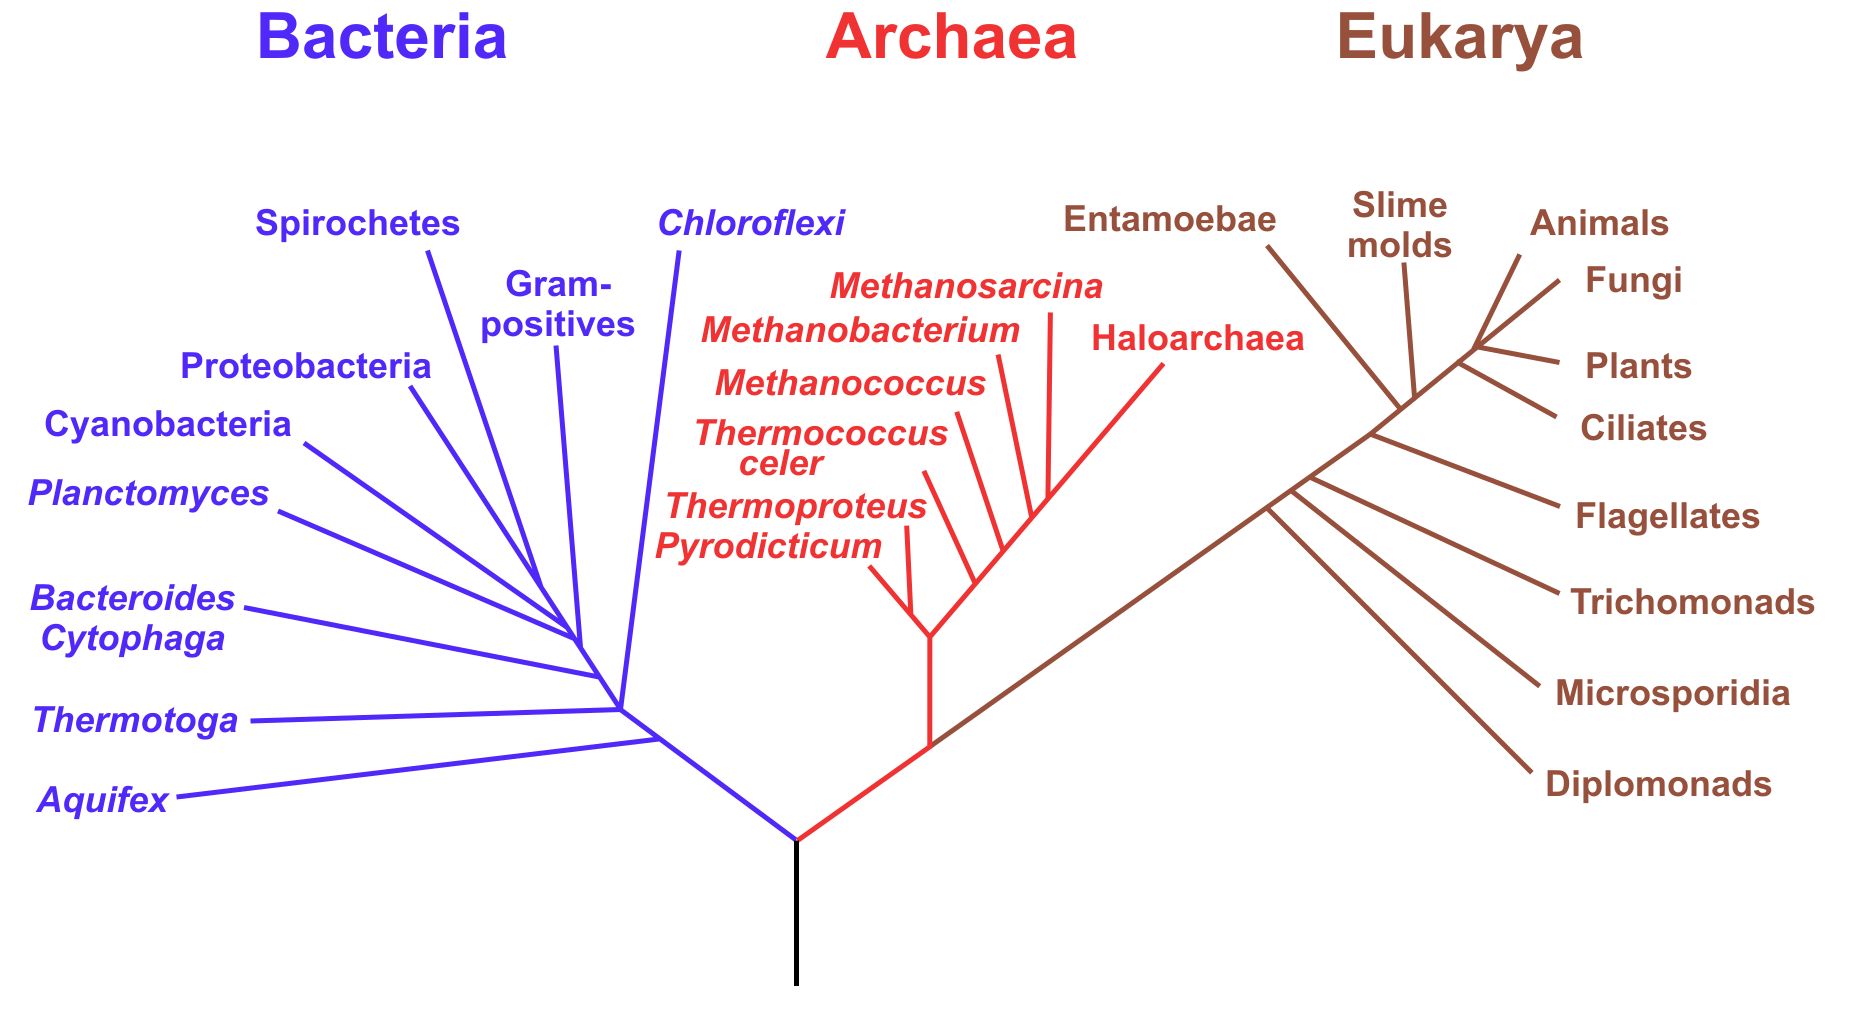
\includegraphics[scale=0.3]{graphics/Phylogenetic_tree.png}
	\caption{A phylogenetic tree is equivalent to a dendrogram.}
	\label{fig:phylogenetic}
\end{figure}

To read a dendrogram, one first finds the many leaves or ends---often these are
labeled---these are the initial clusters. As one goes through the dendrogram
(e.g.\ bottom to top or left to right), clusters get linked, which is depicted
by joining the ends of the initial clusters. This happens until there is exactly
one cluster left. Two ends are closer (or more similar) if they become joined
early on compared to two ends that only become joined near the end of the
dendrogram. 

Let's explain the algorithm using pseudo-code. Instead of outputting a
dendrogram, we will output a list of pairs of the form $(t, [C_1,\dots, C_r])$,
where $t\geq 0$ and each $C_i$ is a finite set of data points. This list will
start with $(0, [C_1,\dots, C_n])$, where each $C_i$ is a singleton, and it will
end with $(t_\infty, [C_1])$, where $C_1$ contains all of the data points. Note
that this data is also equivalent to a dendrogram.

\begin{algorithm}
	\caption{Neighbour joining}\label{alg:neighbour}
	\begin{algorithmic}[1]
		\Require a semimetric $d : \mathscr{F}_m\times \mathscr{F}_m\to \R$ and $n$ data points $x_i\in\R^m$,
		\Ensure a list $D$ equivalent to a dendrogram.
		\State Set $t=0$.
		\State Set $C = \{\{x_1\}, \dots, \{x_n\}\}$.
		\State Set $D = [(t, C)]$.
		\While{$\# C > 1$}
			\State Construct distance matrix $M = (M_{ij})$, with $M_{ij} = d(C_i, C_j)$.
			\State Determine the two closest distinct clusters $C_r$ and $C_s$ from $M$.
			\State Set $t = t + M_{rs}$.
			\State Set $C = (C \setminus \{C_r, C_s\}) \cup \{C_r \cup C_s\}$.
			\State Append to $D$ the pair $(t, C)$.
		\EndWhile
		\State \Return $D$.
	\end{algorithmic}
\end{algorithm}

We will soon go through \Cref{alg:neighbour} on a small example. Unlike
$k$-means, neighbour joining is \emph{deterministic}; that is, it runs the same
every time on the same input. Notice in \Cref{alg:neighbour} that the actual
points $x_i$ do not matter; instead, it's the distances between the points (and
clusters) that matter. Thus, we won't specify points but a \emph{graph}.

\begin{defn}
	A (finite, simple) \textbf{graph} $G$ is a pair of vertices $V = \{v_1,
	\dots, v_n\}$ and edges $E = \{e_1, \dots, e_k\}$, where each $e_i\subseteq
	V$ of size exactly two. Vertices $v_i$ and $v_j$ are \textbf{adjacent},
	written $v_i \sim v_j$, if $\{v_i, v_j\} \in E$.
\end{defn}

Graphs are ubiquitous in mathematics and computer science, and they can be
easily visualised (for a relatively small amount of vertices). Three graphs can
be seen in \Cref{fig:3-graphs}.

\begin{figure}[h]
	\centering
	\begin{minipage}{0.3\textwidth}
		\centering
		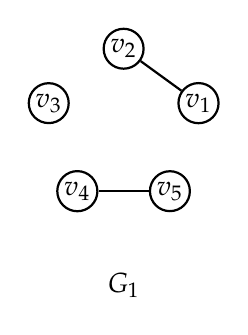
\begin{tikzpicture}
			% Nodes
			\foreach \i in {1,2,3,4,5} {
				\node[circle, draw, fill=white, inner sep=1pt, thick] (node\i) at ({360/5 * (\i - 1) + 18}:1) {$v_{\i}$};
			}
			\node at (0,-2) {$G_1$};
			\draw[thick] (node1) -- (node2);
			\draw[thick] (node4) -- (node5);
		\end{tikzpicture}
	\end{minipage}~
	\begin{minipage}{0.3\textwidth}
		\centering
		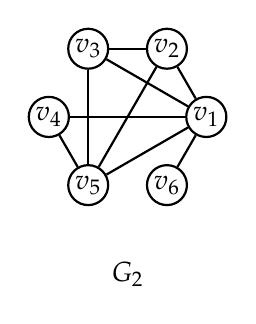
\begin{tikzpicture}
			% Nodes
			\foreach \i in {1,2,3,4,5,6} {
				\node[circle, draw, fill=white, inner sep=1pt, thick] (node\i) at ({360/6 * (\i - 1)}:1) {$v_{\i}$};
			}
			\node at (0,-2) {$G_2$};
			\draw[thick] (node1) -- (node2);
			\draw[thick] (node1) -- (node3);
			\draw[thick] (node1) -- (node4);
			\draw[thick] (node1) -- (node5);
			\draw[thick] (node1) -- (node6);
			\draw[thick] (node2) -- (node3);
			\draw[thick] (node2) -- (node5);
			\draw[thick] (node4) -- (node5);
			\draw[thick] (node3) -- (node5);
		\end{tikzpicture}
	\end{minipage}~
	\begin{minipage}{0.3\textwidth}
		\centering
		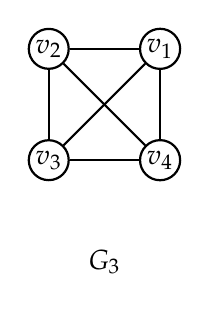
\begin{tikzpicture}
			% Nodes
			\foreach \i in {1,2,3,4} {
				\node[circle, draw, fill=white, inner sep=1pt, thick] (node\i) at ({360/4 * (\i) - 45}:1) {$v_{\i}$};
			}
			\node at (0,-2) {$G_3$};
			\draw[thick] (node1) -- (node2);
			\draw[thick] (node1) -- (node3);
			\draw[thick] (node1) -- (node4);
			\draw[thick] (node2) -- (node3);
			\draw[thick] (node2) -- (node4);
			\draw[thick] (node3) -- (node4);
		\end{tikzpicture}
	\end{minipage}
	\caption{Three different graphs.}
	\label{fig:3-graphs}
\end{figure}

\subsection{A small example of hierarchical clustering}

Instead of writing down or plotting data points, we will write down a distance
matrix. The distance matrix is a symmetric matrix with zeros along the diagonal.
(Why?) The $(i,j)$ entry is equal to the distance between vertices (or clusters)
$v_i$ and $v_j$. Let's consider the following distance matrix.
\begin{center}
	\begin{tabular}{c|cccccc}
		& $v_1$ & $v_2$ & $v_3$ & $v_4$ & $v_5$ & $v_6$ \\ \hline 
		$v_1$ & 0 & 4 & 8 & 1 & 7 & 8 \\
		$v_2$ & 4 & 0 & 6 & 5 & 5 & 6 \\
		$v_3$ & 8 & 6 & 0 & 7 & 2 & 2 \\
		$v_4$ & 1 & 5 & 7 & 0 & 8 & 8 \\
		$v_5$ & 7 & 5 & 2 & 8 & 0 & 1 \\
		$v_6$ & 8 & 6 & 2 & 8 & 1 & 0 
	\end{tabular}
\end{center}

We will apply single- and complete-linkages and cluster the data accordingly.
Because we know how to compute them both given the distances from all pairs of
vertices, we will not recompute our distance matrix each time. Instead we will
draw nine graphs labeled $G_t$ for $t\in \{0, \dots, 8\}$ since the maximal
distance between any two points is $8$. We will include an edge between $v_i$
and $v_j$ in $G_t$ if and only if $d(v_i, v_j)\leq t$. The graph $G_0$ is the
graph on 8 vertices with no edges, and the graph $G_8$ is the graph on 8
vertices where every vertex is adjacent to every other vertex (this is called a
\emph{complete graph}). All of the graphs are shown in \Cref{fig:9-graphs}.

\begin{figure}[h]
	\centering 
	\begin{tikzpicture}
		\node at (0, 2*4) {
		\begin{tikzpicture}
			% Nodes
			\foreach \i in {1,2,3,4,5,6} {
				\node[circle, draw, fill=white, inner sep=1pt, thick] (node\i) at ({360/6 * (\i - 1)}:1) {$v_{\i}$};
			}
			\node at (0, -1.75) {$G_0$};
		\end{tikzpicture}
		};
		\node at (1*4.5, 2*4) {
		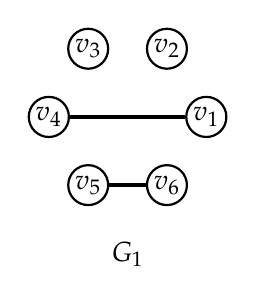
\begin{tikzpicture}
			% Nodes
			\foreach \i in {1,2,3,4,5,6} {
				\node[circle, draw, fill=white, inner sep=1pt, thick] (node\i) at ({360/6 * (\i - 1)}:1) {$v_{\i}$};
			}
			\node at (0, -1.75) {$G_1$};
			\draw[ultra thick] (node1) -- (node4);
			\draw[ultra thick] (node5) -- (node6);
		\end{tikzpicture}
		};
		\node at (2*4.5, 2*4) {
		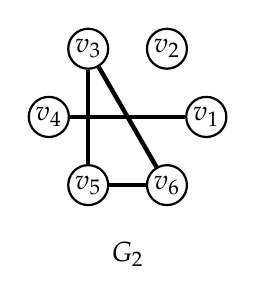
\begin{tikzpicture}
			% Nodes
			\foreach \i in {1,2,3,4,5,6} {
				\node[circle, draw, fill=white, inner sep=1pt, thick] (node\i) at ({360/6 * (\i - 1)}:1) {$v_{\i}$};
			}
			\node at (0, -1.75) {$G_2$};
			\draw[ultra thick] (node1) -- (node4);
			\draw[ultra thick] (node5) -- (node6);
			\draw[ultra thick] (node3) -- (node5);
			\draw[ultra thick] (node3) -- (node6);
		\end{tikzpicture}
		};
		\node at (0, 1*4) {
		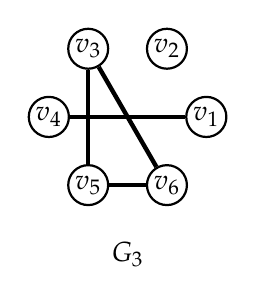
\begin{tikzpicture}
			% Nodes
			\foreach \i in {1,2,3,4,5,6} {
				\node[circle, draw, fill=white, inner sep=1pt, thick] (node\i) at ({360/6 * (\i - 1)}:1) {$v_{\i}$};
			}
			\node at (0, -1.75) {$G_3$};
			\draw[ultra thick] (node1) -- (node4);
			\draw[ultra thick] (node5) -- (node6);
			\draw[ultra thick] (node3) -- (node5);
			\draw[ultra thick] (node3) -- (node6);
		\end{tikzpicture}
		};
		\node at (1*4.5, 1*4) {
		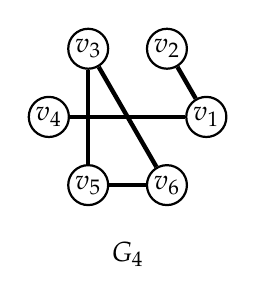
\begin{tikzpicture}
			% Nodes
			\foreach \i in {1,2,3,4,5,6} {
				\node[circle, draw, fill=white, inner sep=1pt, thick] (node\i) at ({360/6 * (\i - 1)}:1) {$v_{\i}$};
			}
			\node at (0, -1.75) {$G_4$};
			\draw[ultra thick] (node1) -- (node4);
			\draw[ultra thick] (node5) -- (node6);
			\draw[ultra thick] (node3) -- (node5);
			\draw[ultra thick] (node3) -- (node6);
			\draw[ultra thick] (node1) -- (node2);
		\end{tikzpicture}
		};
		\node at (2*4.5, 1*4) {
		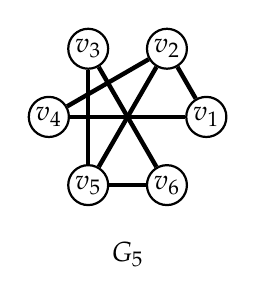
\begin{tikzpicture}
			% Nodes
			\foreach \i in {1,2,3,4,5,6} {
				\node[circle, draw, fill=white, inner sep=1pt, thick] (node\i) at ({360/6 * (\i - 1)}:1) {$v_{\i}$};
			}
			\node at (0, -1.75) {$G_5$};
			\draw[ultra thick] (node1) -- (node4);
			\draw[ultra thick] (node5) -- (node6);
			\draw[ultra thick] (node3) -- (node5);
			\draw[ultra thick] (node3) -- (node6);
			\draw[ultra thick] (node1) -- (node2);
			\draw[ultra thick] (node2) -- (node4);
			\draw[ultra thick] (node2) -- (node5);
		\end{tikzpicture}
		};
		\node at (0*4.5, 0) {
		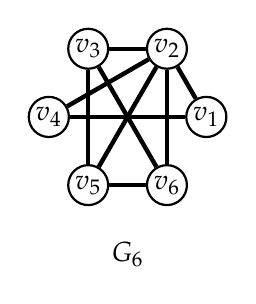
\begin{tikzpicture}
			% Nodes
			\foreach \i in {1,2,3,4,5,6} {
				\node[circle, draw, fill=white, inner sep=1pt, thick] (node\i) at ({360/6 * (\i - 1)}:1) {$v_{\i}$};
			}
			\node at (0, -1.75) {$G_6$};
			\draw[ultra thick] (node1) -- (node4);
			\draw[ultra thick] (node5) -- (node6);
			\draw[ultra thick] (node3) -- (node5);
			\draw[ultra thick] (node3) -- (node6);
			\draw[ultra thick] (node1) -- (node2);
			\draw[ultra thick] (node2) -- (node4);
			\draw[ultra thick] (node2) -- (node5);
			\draw[ultra thick] (node2) -- (node3);
			\draw[ultra thick] (node2) -- (node6);
		\end{tikzpicture}
		};
		\node at (1*4.5, 0) {
		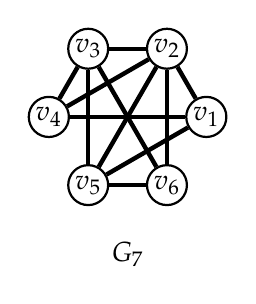
\begin{tikzpicture}
			% Nodes
			\foreach \i in {1,2,3,4,5,6} {
				\node[circle, draw, fill=white, inner sep=1pt, thick] (node\i) at ({360/6 * (\i - 1)}:1) {$v_{\i}$};
			}
			\node at (0, -1.75) {$G_7$};
			\draw[ultra thick] (node1) -- (node4);
			\draw[ultra thick] (node5) -- (node6);
			\draw[ultra thick] (node3) -- (node5);
			\draw[ultra thick] (node3) -- (node6);
			\draw[ultra thick] (node1) -- (node2);
			\draw[ultra thick] (node2) -- (node4);
			\draw[ultra thick] (node2) -- (node5);
			\draw[ultra thick] (node2) -- (node3);
			\draw[ultra thick] (node2) -- (node6);
			\draw[ultra thick] (node1) -- (node5);
			\draw[ultra thick] (node3) -- (node4);
		\end{tikzpicture}
		};
		\node at (2*4.5, 0) {
		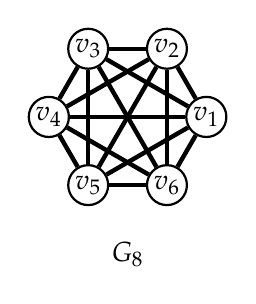
\begin{tikzpicture}
			% Nodes
			\foreach \i in {1,2,3,4,5,6} {
				\node[circle, draw, fill=white, inner sep=1pt, thick] (node\i) at ({360/6 * (\i - 1)}:1) {$v_{\i}$};
			}
			\node at (0, -1.75) {$G_8$};
			\draw[ultra thick] (node1) -- (node4);
			\draw[ultra thick] (node5) -- (node6);
			\draw[ultra thick] (node3) -- (node5);
			\draw[ultra thick] (node3) -- (node6);
			\draw[ultra thick] (node1) -- (node2);
			\draw[ultra thick] (node2) -- (node4);
			\draw[ultra thick] (node2) -- (node5);
			\draw[ultra thick] (node2) -- (node3);
			\draw[ultra thick] (node2) -- (node6);
			\draw[ultra thick] (node1) -- (node5);
			\draw[ultra thick] (node3) -- (node4);
			\draw[ultra thick] (node1) -- (node3);
			\draw[ultra thick] (node1) -- (node6);
			\draw[ultra thick] (node4) -- (node5);
			\draw[ultra thick] (node4) -- (node6);
		\end{tikzpicture}
		};
	\end{tikzpicture}
	\caption{The 9 graphs visualising the possible clustering of the 8 vertices.}
	\label{fig:9-graphs}
\end{figure}


Now we will produce dendrograms, one for the single-linkage and one for the
complete-linkage. There are two concepts in Graph Theory that we can use to
determine these dendrograms. 

\begin{defn}
	Two vertices $v_i$ and $v_j$ of a graph $G$ are \textbf{connected} if there
	exists a sequence of adjacent vertices of the form $v_i = v_0 ~ v_1 ~ \cdots
	~ v_{\ell} = v_j$.
\end{defn}

\begin{defn}
	A subset $S$ of vertices of a graph $G$ form a \textbf{clique} if for all
	distinct $v_i, v_j\in S$, the edge $\{v_i, v_j\}$ is in $G$. 
\end{defn}

Let's consider the graphs in \Cref{fig:9-graphs} again. Using single-linkage, we
know that vertices $v_i$ and $v_j$ lie in the same cluster if and only if $v_i$
and $v_j$ are connected. Therefore, we have exactly one cluster starting at
$G_5$ using single-linkage. Using complete-linkage, we know that vertices
$\{v_{i_1}, \dots, v_{i_{\ell}}\}$ form a cluster if and only if they form a
clique. Hence, we have exactly one cluster starting at $G_8$ using
complete-linkage. The dendrograms can be seen in
\Cref{fig:dendrogram-slink,,fig:dendrogram-clink}. 

% \afterpage{\clearpage}

\begin{figure}[h]
	\centering 
	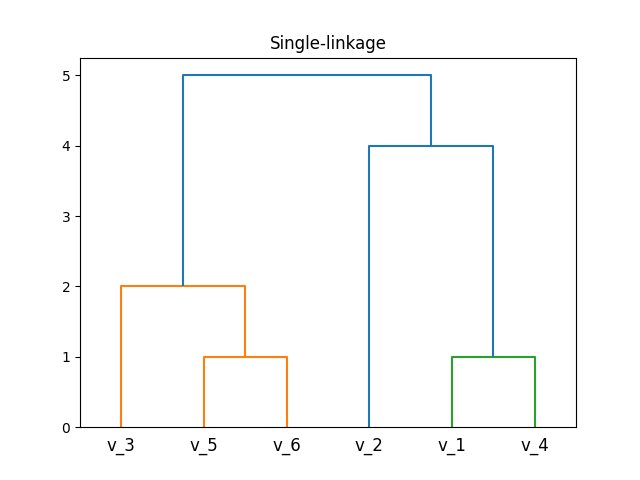
\includegraphics[scale=0.75]{graphics/slink.png}
	\caption{The dendrogram corresponding to the graphs in \Cref{fig:9-graphs} using single-linkage.}
	\label{fig:dendrogram-slink}	
\end{figure}

\begin{figure}[h]
	\centering 
	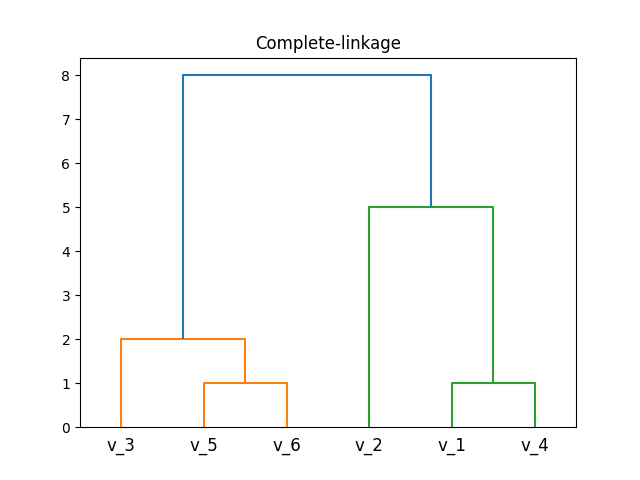
\includegraphics[scale=0.75]{graphics/clink.png}
	\caption{The dendrogram corresponding to the graphs in \Cref{fig:9-graphs} using complete-linkage.}
	\label{fig:dendrogram-clink}	
\end{figure}

































\newpage

\begin{bibdiv}
\begin{biblist}
	\bib{BreastCancer}{article}{
		title={Breast cancer classification and prognosis based on gene expression profiles from a population-based study},
		author={Sotiriou, Christos},
		author={Neo, Soek-Ying},
		author={McShane, Lisa M.},
		author={Korn, Edward L.},
		author={Long, Philip M.},
		author={Jazaeri, Amir},
		author={Martiat, Philippe},
		author={Fox, Steve B.},
		author={Harris, Adrian L.},
		author={Liu, Edison T.},
		journal={Proceedings of the National Academy of Sciences},
		volume={100},
		number={18},
		pages={10393--10398},
		year={2003},
		publisher={National Acad Sciences},
	}

	\bib{FM/90}{article}{
		author={Frankl, Peter},
		author={Maehara, Hiroshi},
		title={Some geometric applications of the beta distribution},
		journal={Ann. Inst. Statist. Math.},
		volume={42},
		date={1990},
		number={3},
		pages={463--474},
		issn={0020-3157},
	}

	\bib{Google}{article}{
		author={Google},
		title={What is Clustering?}
		date={2023},
		status={date accessed: 16 Oct.\ 2023. \url{https://developers.google.com/machine-learning/clustering/overview}},
	}

	\bib{HPIM/12}{article}{
		author={Har-Peled, Sariel},
		author={Indyk, Piotr},
		author={Motwani, Rajeev},
		title={Approximate nearest neighbor: towards removing the curse of
		dimensionality},
		journal={Theory Comput.},
		volume={8},
		date={2012},
		pages={321--350},
		review={\MR{2948494}},
		doi={10.4086/toc.2012.v008a014},
	}

	\bib{ILA}{book}{
		author={Margalit, Dan},
		author={Rabinoff, Joseph},
		title={Interactive Linear Algebra},
		date={2019},
		status={\url{https://textbooks.math.gatech.edu/ila/}},
	}

	\bib{Shlens}{unpublished}{
		author={Shlens, Jonathon},
		title={A tutorial on principal component analysis},
		date={2014},
		status={\href{https://arxiv.org/abs/1404.1100}{\texttt{arXiv:1404.1100}}},
	}

	\bib{YLDW/21}{unpublished}{
      title={How to reduce dimension with PCA and random projections?}, 
      author={Fan Yang and Sifan Liu and Edgar Dobriban and David P. Woodruff},
      year={2021},
      status={\href{https://arxiv.org/abs/2005.00511}{\texttt{arXiv:2005.00511}}}, 
	}
\end{biblist}
\end{bibdiv}

\end{document}